\chapter{Konzept}
\section{Aufbau der Software}
    Die im vorherigen Kapitel dargestellten Use-Case Diagramm und den daraus abgeleiteten Anforderungen, werden in diesem Kapitel zum Aufbau einer Architektur verwendet.
    Hierbei wurde zunächst das Systemdiagramm aus dem Use-Case Diagramm (Abbildung \ref{fig:use-case}) abgeleitet (siehe Abbildung \ref{fig:system_all}).
    
    Die Akteure (\emph{Netwerk-, Systemadministrator} und \emph{Security Auditor}) konnten direkt aus dem Use-Case Diagramm übernommen werden.
    Sie stellen die mit dem System interagierende Nutzer dar und interagieren direkt mit einem Frontend.
    Es erfolgt eine klare Trennung zwischen Backend und Frontend damit Logik und Visualisierung voneinander unabhängig implementiert werden können.
    
    Das \emph{Backend} kommuniziert, durch eine Proxy, mit dem Client und empfängt die gesendeten Nachrichten. Anschließend verarbeitet es diese und leitet die verarbeiteten Nachrichten an den Broker weiter. Sobald eine Antwort zurück kommt, wird diese erneut verarbeitet und anschließend veröffentlicht.
    Die Hauptaufgaben des Backends sind die Datenhaltung (z.B.: Speicherung der Nachrichten, Verwalten der Clients) und die Verwaltung des Nachrichtenflusses zwischen allen beteiligten Kommunikationspartnern.
    
    Das \emph{Frontend} hingegen, dient nur zur Visualisierung der Nachrichten und Clients sowie zur Interaktion mit dem Nutzer. Hierbei bezieht es die gespeicherten und neu eintreffenden Nachrichten vom Backend.
    \begin{figure}[h]%h=direkt danach t=top b=bottom
        \centering
        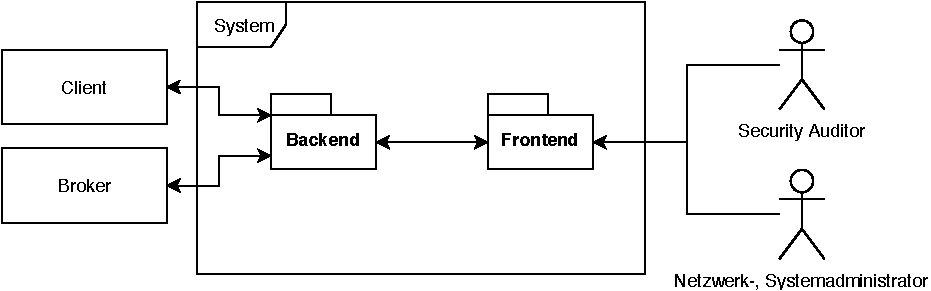
\includegraphics[width=14cm]{tex/bilder/4_konzept/Systemdiagram.pdf}
        \captionof{figure}{Systemdiagramm}
        \label{fig:system_all}
    \end{figure}
    
    Abbildung \ref{fig:system_backend} zeigt eine Verfeinerung des Backends.Sobald ein Client eine Verbindung zum Broker aufbaut, werden zwei virtuelle Clients erzeugt.
    
    Einer der Clients (\emph{ClientOut}) repräsentiert das tatsächliche Gerät und täuscht dies dem externen Broker gegenüber vor. Er übernimmt somit die Übertragung der Nachrichten zwischen dem Broker des Proxies und dem externen Broker. Daraus resultiert, dass für den Fall, das Nachrichten von dem externen Broker an den \emph{ClientOut} gesendete werden, diese auch dem echten Gerät übermittelt werden müssen. Dazu dient der zweite virtuelle Client (\emph{ClientIn}). Dieser sendet die vom ersten Client erhaltene Nachricht an den internen Broker weiter. Mit der Folge, dass dieser anschließend die Nachricht veröffentlicht. Dabei muss sichergestellt werde, dass die erhaltene Nachricht nicht erneut nach außen gesendet wird.
    
    Der ClientManager übersetzt die externe Clients zu den dazugehörigen \emph{ClientIn} und \emph{ClientOut} Instanzen. Damit wird sichergestellt, dass die eine Kommunikation mit dem externen Broker stattfinden kann.
    \begin{figure}[h]%h=direkt danach t=top b=bottom
        \centering
        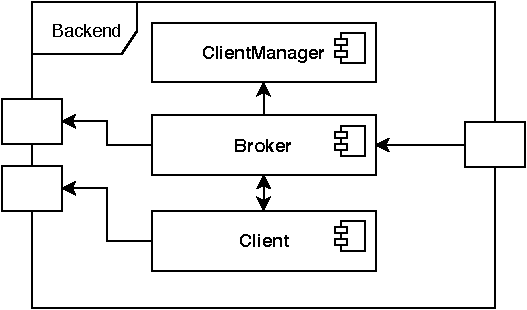
\includegraphics[width=8cm]{tex/bilder/4_konzept/Systemdiagramm_Konzept_Backend.pdf}
        \captionof{figure}{Komponentendiagramm Backend}
        \label{fig:system_backend}
    \end{figure}
    
    Abbildung \ref{fig:system_frontend} stellt die Komponenten des Frontends dar. Alle drei Komponenten sind voneinander unabhängig und arbeiten mit unabhängigen Informationen.
    
    Die Clients Komponente enthält die Informationen der virtuellen Clients (\emph{ClientIn} und \emph{ClientOut}). Diese werden sobald der Nutzer die Seite besucht vom Backend geladen und anschließend angezeigt. Sie ermöglicht ebenfalls die Konfigurieren der abzufangenden Kommunikation pro Gerät.
    
    Die NewMessages Komponente ermöglicht das Erzeugen von neuen Nachrichten auf der Seite des Frontends und überträgt am Ende alle Informationen an das Backend, wo diese weiter verarbeitet (z.B.: versendet) werden.
    
    Der Interceptor ist für die Anzeige der abgefangen Nachrichten zuständig. Zu Beginn werden alle bestehenden Nachrichten abgefangen und, um das wiederholte laden der Webseite zu verhindern und die Aktualität zu gewährleisten, dynamisch alle weiteren eingehenden Nachrichten nachgeladen. Um die Anzeige noch weiter zu strukturieren, werden ebenfalls verschiedene Filter zur Verfügung gestellt, welche auf die Nachrichteninhalte angewendet werden können.
    \begin{figure}[h]%h=direkt danach t=top b=bottom
        \centering
        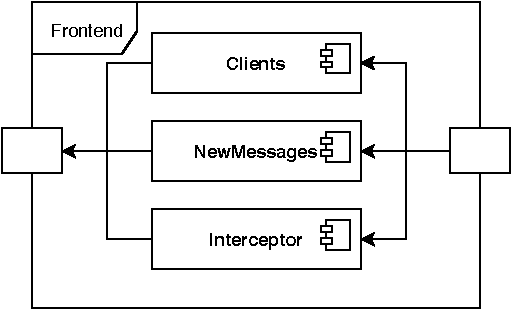
\includegraphics[width=8cm]{tex/bilder/4_konzept/Systemdiagramm_Konzept_Frontend.pdf}
        \captionof{figure}{Komponentendiagramm Frontend}
        \label{fig:system_frontend}
    \end{figure}

\section{Prozess}
In diesem Abschnitt wird die Kommunikation zwischen den Systeme behandelt.
    \begin{figure}[h]%h=direkt danach t=top b=bottom
        \centering
        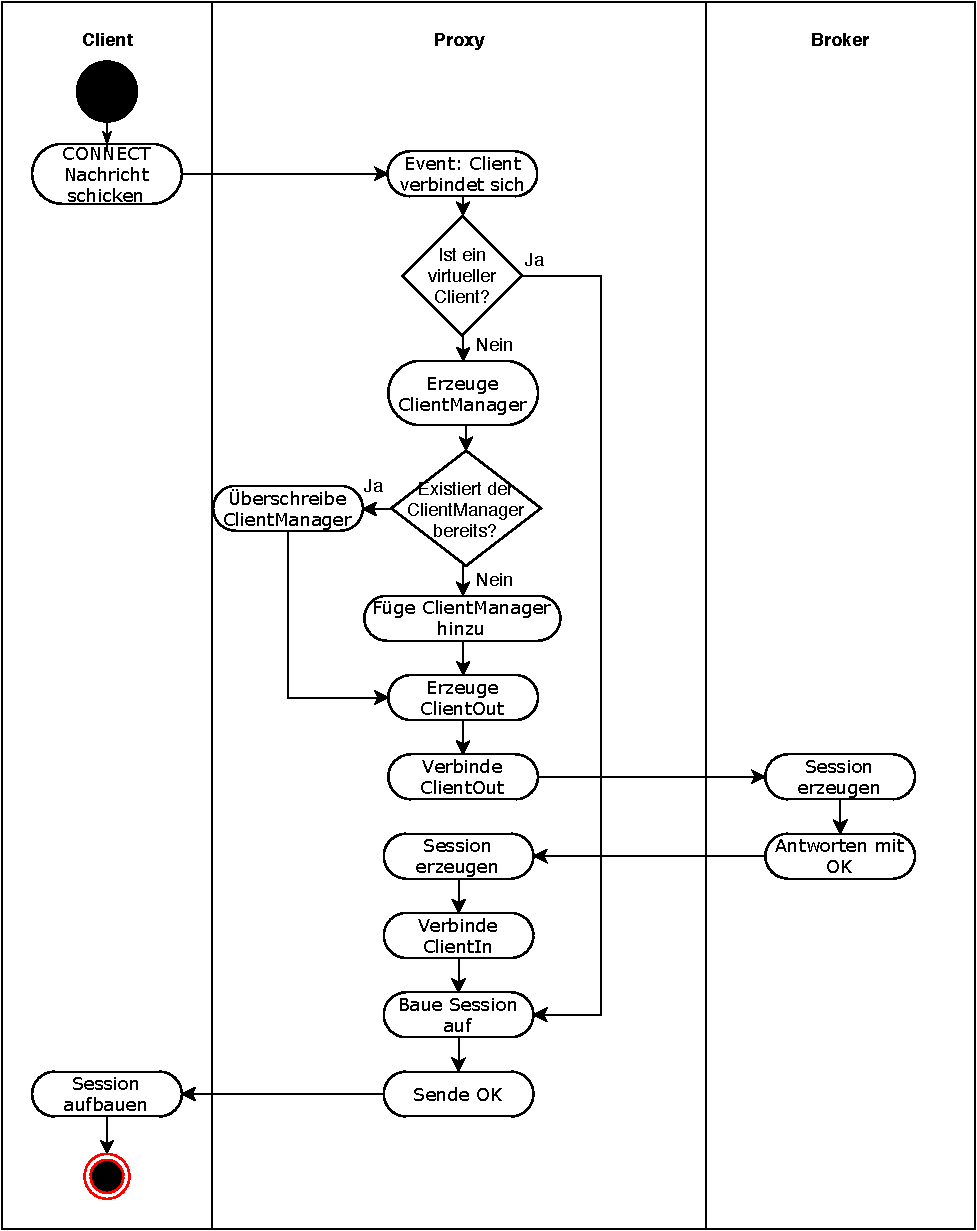
\includegraphics[width=10cm]{tex/bilder/4_konzept/Activity_Connect.pdf}
        \captionof{figure}{Komponentendiagramm Frontend}
        \label{fig:system_frontend}
    \end{figure}
    \begin{figure}[h]%h=direkt danach t=top b=bottom
        \centering
        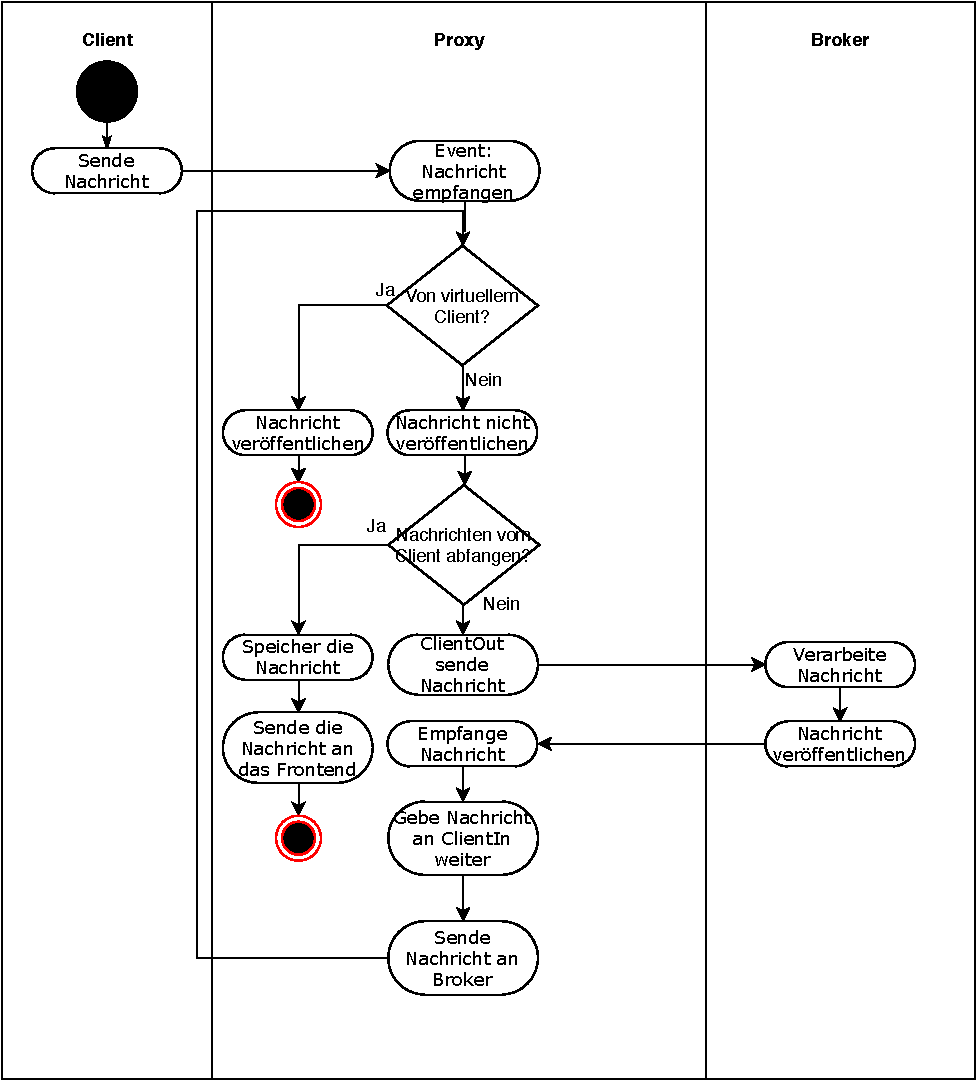
\includegraphics[width=10cm]{tex/bilder/4_konzept/Activity_Message.pdf}
        \captionof{figure}{Komponentendiagramm Frontend}
        \label{fig:system_frontend}
    \end{figure}
    \begin{figure}[h]%h=direkt danach t=top b=bottom
        \centering
        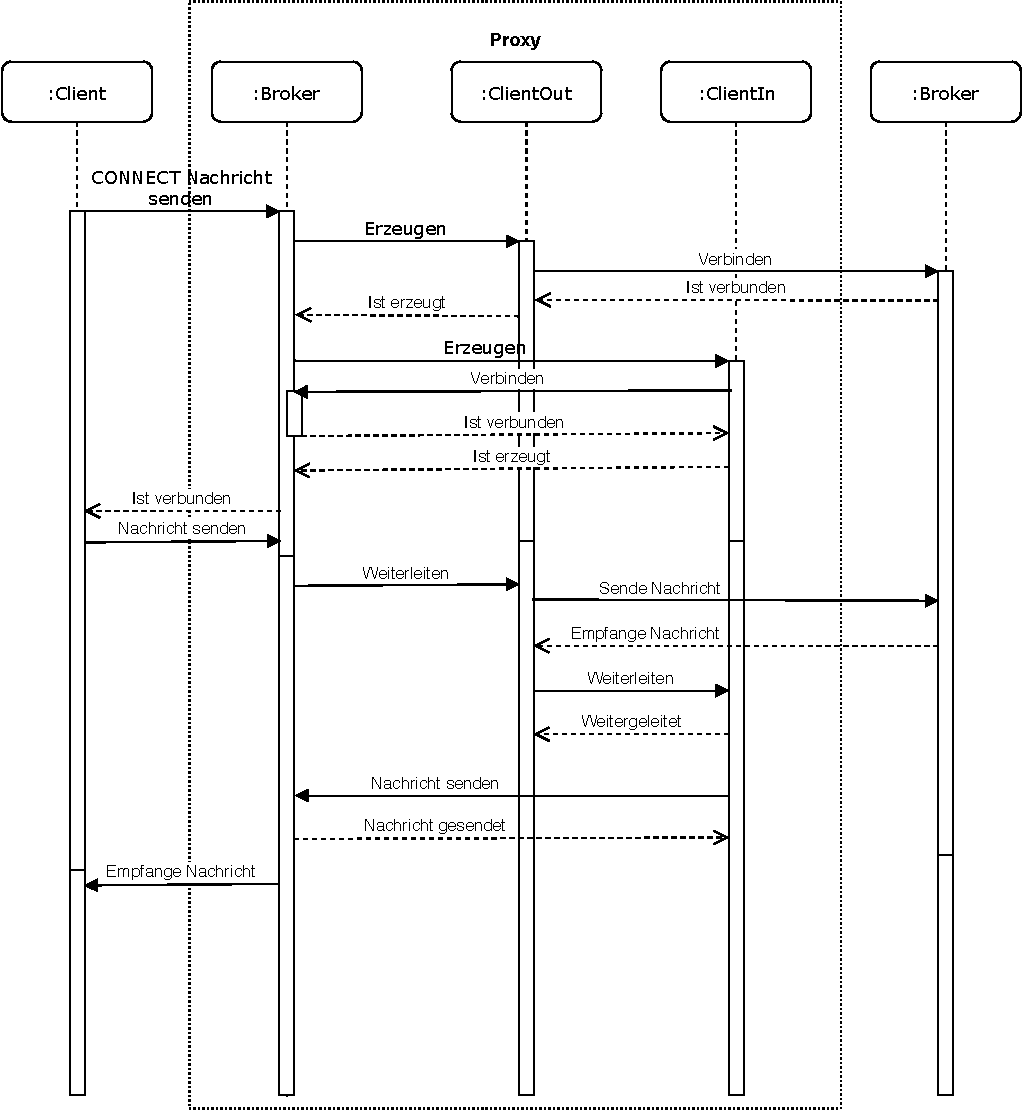
\includegraphics[width=12cm]{tex/bilder/4_konzept/Sequenz.pdf}
        \captionof{figure}{Komponentendiagramm Frontend}
        \label{fig:system_frontend}
    \end{figure}
%Aktivitätsdiagramm
%Sequenzdiagramm
